\documentclass{beamer}
\usepackage{graphicx}
\usepackage[T2A]{fontenc}    
\usepackage[utf8]{inputenc}  
\usepackage[english,russian]{babel}
\usepackage{amsmath}
\usepackage{wrapfig}
\renewcommand{\normalsize}{\small}
\begin{document}
\begin{frame}
    \begin{flushright}
        Мера количества информации по Шеннону
    \end{flushright}
    Мера Хартли подходит лишь для систем с равноверотяными состояниями. Если состояние системы S не равновероятны, исопльзуют меру Шеннона: \\
    
    \begin{wrapfigure}{r}{0.2\textwidth}
        \centering
        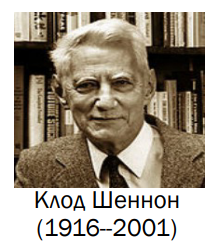
\includegraphics{img1.png} 
    \end{wrapfigure}
    
    \[
    i(S) = -\sum_{i=1}^{N} p_i \cdot \log_2 p_i,
    \]
    
    где N - число системы, 
    $p_i$ - вероятность того, что система S находится в
    состоянии i (сумма всех $p_i$ равна 1)
    \begin{center}
        Формула Хартли является частным случаем формулы Шеннона!
    \end{center}
    \textbf{Пример 1.} Количество информации в акте подбрасывания обычной монеты по формуле Хартли равно $log_2 2$ = 1 бит.  По формуле Шеннона получим то же: $i_s1 = -0.5*log_2 0.5 = 1$ бит.\\
    \textbf{Пример 2.} При подбрасывании монеты со смещённым центром тяжести количество непредсказуемости становится меньше: $i_s2 = -0.75 * log_2 0.75 - 0.25 * log_2 0.25 \approx 0,8$ бит.
\end{frame}
\begin{frame}
    \begin{flushright}
        Пример использования меры Шеннона
    \end{flushright}
    Шулер наугад вытаскивает одну карту из стопки, содержащей 9 известных ему карт: 3
    джокера, 3 туза, 1 король, 1 дама и 1 валет. Какое количество информации для шулера
    содержится в этом событии s? \\
    
    Вероятность вытащить \[
    \left\{
    \begin{array}{ll}
    \text{джокера} \\
    \text{туза} \\
    \text{короля} \\
    \text{даму} \\
    \text{валета}
    \end{array}
    \right\}
    \text{ равна }
    \left\{
    \begin{array}{ll}
    \frac{3}{9} = \frac{1}{3} \\
    \frac{3}{9} = \frac{1}{3} \\
    \frac{1}{9} \\
    \frac{1}{9} \\
    \frac{1}{9}
    \end{array}
    \right.
    \]
    
    Количество информации, выраженное в тритах, равно:
    \[
    i(s) = -\left(
    \frac{1}{3} \cdot \log_3 \frac{1}{3} 
    + \frac{1}{3} \cdot \log_3 \frac{1}{3} 
    + \frac{1}{9} \cdot \log_3 \frac{1}{9} 
    + \frac{1}{9} \cdot \log_3 \frac{1}{9} 
    + \frac{1}{9} \cdot \log_3 \frac{1}{9}
    \right) =
    \]
    \[
    = \frac{1}{3} + \frac{1}{3} + \frac{2}{9} + \frac{2}{9} + \frac{2}{9} = 1 \frac{1}{3} \approx \log_3 5 \quad \text{vs} \quad \log_3 14
    \] 
\end{frame}
\begin{frame}
    \begin{flushright}
        Нестрогий вывод формулы Шеннона
    \end{flushright}
    \textbf{Задача.} Монета имеет смещённый центр тяжести. Вероятность выпадения «орла» – 0,25, вероятность выпадения «решки» – 0,75. Какое количество информации содержится в одном подбрасывании? 
    \textbf{Решение.}
    \begin{itemize}
        \item Пусть монета была подброшена N раз (N→∞), из которых «решка» выпала M раз, «орёл» — K раз (очевидно, что N = M + K). 
        \item Количество информации в N подбрасываниях: $i_N$ = M*i(«решка») + K*i(«орёл»). 
        \item Тогда среднее количество информации в одном подбрасывании: $i_1=i_N/N$ = = (M/N)*i(«решка»)+(K/N)*i(«орёл») = p(«решка»)*i(«решка»)+p(«орёл»)*i(«орёл»).
        \item Подставив формулу Шеннона для i, окончательно получим: $i_1$ = = -p(«решка»)*$log_x p$p(«решка») - p(«орёл»)*$log_x p$p(«орёл»)$\approx 0.8$ бит.
    \end{itemize}
\end{frame}
\begin{frame}
    \begin{flushright}
        Приставки для единиц измерения
количества информации/данных: проблема
    \end{flushright}
    \begin{minipage}{0.45\textwidth}
        \centering
        \textbf{Linux Ubuntu 14} \\
        \vspace{0.5em}
        \includegraphics[width=\textwidth]{image2.png}
    \end{minipage}%
    \hfill
    \begin{minipage}{0.45\textwidth}
        \centering
        \textbf{Microsoft Windows 7} \\
        \vspace{0.5em}
        \includegraphics[width=\textwidth]{image3.png}
    \end{minipage} \\
    \begin{center}
        33 097 216 байт — это 33,1 МБ или 31,5 МБ?
    \end{center}
\end{frame}
\begin{frame}
    \begin{flushright}
        Приставки для единиц измерения
количества информации/данных: решение
    \end{flushright}
    1. IEEE 1541-2002 – Институт инженеров по электротехнике и радиоэлектронике. \\
    2. ISO/IEC 80000-13:2008 – Международная организация по стандартизации. \\
    3. ГОСТ IEC 60027-2-2015 – Международная электротехническая комиссия. \\
    \begin{table}
    \centering
    \begin{tabular}{|c|c|c|}
        \hline
        Приставки единиц СИ & Новые двоичные префиксы & $\Delta,  $,  \\ \hline
        килобайт (kB) = $10^3$ байт        & кибибайт (KiB, КиБ) = $2^(10)$ байт         & 2         \\ \hline
        мегабайт (MB) = $10^6$ байт        & мебибайт (MiB, МиБ) = $2^(20)$ байт         & 5         \\ \hline
        гигабайт (GB) = $10^9$ байт        & гибибайт (GiB, ГиБ) = $2^(30)$ байт         & 7         \\ \hline
        терабайт (TB) = $10^(12)$ байт       & тебибайт (TiB, ТиБ) = $2^(40)$ байт         & 10         \\ \hline
    \end{tabular}
\end{table}
\textbf{Краткое обозначение битов и байтов: }  b = bit = бит, B = Б = байт
 1024 B = 1024 Б = 8192 b = 8192 бит = 8 Кибит = 1 КиБ = 1 KiB
\end{frame}
\end{document}